% !TeX root = surprises.tex

\chapter{Dreiteilung eines Winkels}\label{c.trisect}

%%%%%%%%%%%%%%%%%%%%%%%%%%%%%%%%%%%%%%%%%%%%%%%%%%%%%%%%%%%%%%%

Es ist unmöglich, einen beliebigen Winkel nur mit Lineal und Zirkel zu dreiteilen (den Winkel in drei gleiche Teile zu zerlegen). Die Dreiteilung erfordert die Konstruktion von Kubikwurzeln, aber ein Lineal und ein Zirkel können nur Längen konstruieren, die aus ganzen Zahlen, den vier arithmetischen Operatoren und Quadratwurzeln gebildet sind. Dies wurde von Pierre Wantzel im Jahr 1837 bewiesen. Dennoch versuchen unzählige Amateure weiterhin, einen Winkel zu dreiteilen. Ihre Konstruktionen sind Annäherungen, auch wenn sie davon überzeugt sind, dass die Konstruktionen korrekt sind. Abschnitt~\ref{s.trisect-approx} stellt zwei solcher Konstruktionen vor, entwickelt Formeln für die Winkel und zeigt die Fehler in den Näherungen.

Die griechischen Mathematiker entdeckten, dass man Winkel dreiteilen kann, wenn man andere Instrumente zulässt. Abschnitt~\ref{s.neusis} erklärt eine Konstruktion von Archimedes\index{Archimedes}, die ein einfaches Instrument namens \emph{neusis} verwendet, und Abschnitt~\ref{s.neusis-doubling} zeigt, wie man einen Würfel mit Hilfe der neusis verdoppelt. Abschnitt~\ref{s.q} stellt eine Konstruktion für die Dreiteilung durch Hippias\index{Hippias} unter Verwendung eines Instruments namens \emph{quadratrix} vor. Der Rest des Kapitels enthält einen Beweis für die Unmöglichkeit der Dreiteilung eines Winkels. Abschnitt~\ref{s.trisect-constructible} charakterisiert konstruierbare Zahlen, Abschnitt~\ref{s.trisect-poly} setzt konstruierbare Zahlen mit Wurzeln von Polynomen in Beziehung und Abschnitt~\ref{s.trisect-impossible} verwendet diese Theorie, um zu zeigen, dass die Dreiteilung eines Winkels und die Verdopplung eines Würfels unmöglich sind.

%%%%%%%%%%%%%%%%%%%%%%%%%%%%%%%%%%%%%%%%%%%%%%%%%%%%%%%%

\section{Ungefähre Dreiteilungen}\label{s.trisect-approx}

\subsection{Erste annähernde Dreiteilung}\index{Trisection of an angle!approximation}\label{sub.trisect-approx1}

\noindent\textbf{Konstruktion:}
Sei $\theta=\angle AOB$ ein beliebiger Winkel und nehme ohne Verlust der Allgemeinheit an, dass $A,B$ auf einem Einheitskreis liegen, dessen Mittelpunkt $O$ ist. Halbiere $\angle AOB$ und sei $C$ der Schnittpunkt der Winkelhalbierenden mit dem Einheitskreis. Sei $D$ der Mittelpunkt der $\overline{OA}$ und sei $T$ der Mittelpunkt der $\overline{DC}$. Bezeichne den Winkel $\angle DOT$ mit $\phi$ (Fig.~\ref{f.trisect-first-approx-1}).

\begin{figure}[ht]
\begin{center}
\begin{tikzpicture}[scale=.6]
\coordinate (O) at (0,0)
  node[left] {$O$}
  node[above right,xshift=14pt,yshift=16pt] {\sm{\theta/2}}
  node[right,xshift=18pt,yshift=4pt] {\sm{\theta/2}};
\coordinate (A) at (9cm,0);
\node[right] at (A) {$A$};
\coordinate (B) at (60:9);
\node[above] at (B) {$B$};
\draw (A) arc(0:60:9);
\draw (B) -- (O) -- (A);
\coordinate (C) at (30:9);
\node[right] at (C) {$C$};
\draw (O) -- node[above] {$1$} (C);
\coordinate (D) at (4.5,0);
\node[below] at (D) {$D$};
\coordinate (T) at ($(D)!.5!(C)$);
\draw (D) -- node[left] {$a$} (T) -- node[left] {$a$} (C);
\node[right] at (T) {$T$};
\draw (O) -- (T);
\draw (	1,0) arc (0:30:1);
\draw (30:.8) arc (30:60:.8);
\draw (2,0) arc (0:20:2);
\node[above right] at (2.1,0.1) {\sm{\phi}}; 

\draw[<->] (0,-1) -- node[fill=white] {$1/2$} +(4.5,0);
\draw[<->] (4.5,-1) -- node[fill=white] {$1/2$} +(4.5,0);
\end{tikzpicture}
\end{center}
\caption{Erste annähernde Dreiteilung (1)}\label{f.trisect-first-approx-1}
\end{figure}

\begin{theorem}
\[\tan\phi =\frac{2\sin(\theta/2)}{1+2\cos(\theta/2)}\,.\]
\end{theorem}

\begin{proof} Abbildung~\ref{f.trisect-first-approx-2} ist ein Ausschnitt aus Abb.~\ref{f.trisect-first-approx-1} und enthält zusätzliche Anmerkungen.

Sei $\overline{CF}$ die Senkrechte zu $\overline{OA}$, die $\overline{OA}$ in $F$ schneidet. Da $\overline{OC}=1$ ist, ist $\overline{CF}=\sin (\theta/2)$ und $\overline{OF}=\cos(\theta/2)$. Sei $\overline{TE}$ die Senkrechte zu $\overline{OA}$, die $\overline{OA}$ in $E$ schneidet.

$T$ ist der Mittelpunkt von $\overline{DC}$, also $\overline{DT}=\overline{TC}=a$. Aber $\overline{FT}$ ist der Median zur Hypotenuse eines rechtwinkligen Dreiecks, also ist $\overline{FT}=a$ und somit ist das $\triangle DTF$ isozyklisch. Daraus folgt, dass $\overline{TE}$ sowohl der Median als auch die Höhe von $\overline{DF}$ ist. Aus dem Diagramm ist das leicht zu erkennen:

\begin{figure}[ht]
\begin{center}
\begin{tikzpicture}[scale=.9]
\coordinate (O) at (0,0)
  node[left] {$O$}
  node[right,xshift=24pt,yshift=5pt] {\sm{\theta/2}};
\coordinate (A) at (9cm,0);
\node[right] at (A) {$A$};
\draw (O) -- (A);
\coordinate (C) at (30:9);
\node[right] at (C) {$C$};
\draw (O) -- node[above] {$1$} (C);
\coordinate (D) at (4.5,0);
\node[below] at (D) {$D$};
\coordinate (T) at ($(D)!.5!(C)$);
\draw (D) -- node[left] {$a$} (T) -- node[left] {$a$} (C);
\node[right] at (T) {$T$};
\draw (O) -- (T);
\draw (	1,0) arc (0:30:1);
\draw (2,0) arc (0:20:2);
\node[above right] at (1.9,0.1) {\sm{\phi}}; 

\coordinate (E) at (T |- A);
\draw[thick,dashed] (T) -- node[right] {$h$}
  (E) node[below] {$E$};
\draw[rotate=90] (E) rectangle +(7pt,7pt);

\coordinate (F) at (C |- A);
\draw[thick,dashed] (C) --
  node[right] {$\sin (\theta/2)$} (F) node[below] {$F$};
\draw[rotate=90] (F) rectangle +(7pt,7pt);

\draw[thick,dashed] (T) -- node[right] {$a$} (F);

\draw[<->] ($(O)+(0,-1)$) --
  node[fill=white] {$1/2$} +(4.5,0);
\draw[<->] ($(O)+(0,-1.8)$) --
  node[fill=white] {$\cos (\theta/2)$} ($(F)+(0,-1.8)$);
\draw[<->] ($(D)+(0,-2.6)$) --
  node[fill=white] {$\left(\cos (\theta/2)\!-\! (1/2)\right)$} 
  ($(F)+(0,-2.6)$);
\draw[<->] ($(O)+(0,-3.4)$) --
  node[fill=white] {$(1/2)+(1/2)\left(\cos (\theta/2)\! -\! (1/2)\right)$} 
  ($(E)+(0,-3.4)$);
\end{tikzpicture}
\end{center}
\caption{Erste annähernde Dreiteilung (2)}\label{f.trisect-first-approx-2}
\end{figure}
\[
\overline{OE}=\frac{1}{2} + \frac{1}{2}\left(\cos \frac{\theta}{2}-\frac{1}{2}\right)\,.
\]
Berechnen Sie die Länge $2a=\overline{CD}$ mit Hilfe des Satzes von Pythagoras in $\triangle DCF$:
\begin{eqnarray*}
(2a)^2 &=&  \left(\cos \frac{\theta}{2}-\frac{1}{2}\right)^2+\sin^2\frac{\theta}{2}\,.
\end{eqnarray*}

Die Länge $h=\overline{TE}$ kann aus dem Satz des Pythagoras berechnet werden in $\triangle DTE$:
\begin{eqnarray*}
a^2 &=& h^2 + \left[\frac{1}{2}\left(\cos \frac{\theta}{2}-\frac{1}{2}\right)\right]^2\\
h^2&=&\frac{1}{4}\left(\cos \frac{\theta}{2}-\frac{1}{2}\right)^2+\frac{1}{4}\sin^2\frac{\theta}{2}-\left[\frac{1}{2}\left(\cos \frac{\theta}{2}-\frac{1}{2}\right)\right]^2=
\frac{1}{4}\sin^2\frac{\theta}{2}\\
h&=&\frac{1}{2}\sin\frac{\theta}{2}\\
\tan\phi &=&\frac{h}{\overline{OE}}=\displaystyle\frac{\displaystyle\frac{1}{2}\sin\frac{\theta}{2}}{\displaystyle\frac{1}{2}+\frac{1}{2}\left(\cos \frac{\theta}{2}\! -\! \frac{1}{2}\right)}
=\frac{\displaystyle2\sin\frac{\theta}{2}}{\displaystyle 1+2\cos\frac{\theta}{2}}\,.
\end{eqnarray*}                  
\end{proof}

Dies ist eine Annäherung an eine Dreiteilung $\phi=\theta/3$. Für $\theta=60^\circ$:
\[
\tan^{-1}\left(\frac{2\sin 30^\circ}{1+2\cos 30^\circ}\right)=
\tan^{-1}0.366\approx 20.1^\circ\approx 20^\circ\,.
\]

Tabelle~\ref{t.trisect-first} zeigt die Fehler für eine Reihe von spitzen Winkeln. Der Fehler ist bei kleinen Winkeln relativ gering und steigt bei $85^\circ$ auf $1\%$ an.

\begin{table}[t]
\caption{Fehler bei der ersten approximativen Dreiteilung}\label{t.trisect-first}
\[
%
\begin{array}{r@{\hspace{5mm}}r@{\hspace{5mm}}r@{\hspace{5mm}}r@{\hspace{5mm}}r}
\hline
\noalign{\smallskip}
\theta ({}^\circ) & \theta/3 ({}^\circ)& \tan^{-1} \phi ({}^\circ) & \mathrm{Fehler} ({}^\circ) & \mathrm{Fehler (\%)}\\\hline
\noalign{\smallskip}
  5 &    1.667 &    1.667  &     0.000 &    0.004 \\
 10 &    3.333 &    3.334  &     0.000 &    0.014 \\
 15 &    5.000 &    5.002  &     0.002 &    0.032 \\
 20 &    6.667 &    6.670  &     0.004 &    0.057 \\
 25 &    8.333 &    8.341  &     0.007 &    0.088 \\
 30 &   10.000 &   10.013  &     0.013 &    0.128 \\
 35 &   11.667 &   11.687  &     0.020 &    0.174 \\
 40 &   13.333 &   13.364  &     0.030 &    0.228 \\
 45 &   15.000 &   15.043  &     0.043 &    0.289 \\
 50 &   16.667 &   16.726  &     0.060 &    0.358 \\
 55 &   18.333 &   18.413  &     0.080 &    0.435 \\
 60 &   20.000 &   20.104  &     0.104 &    0.520 \\
 65 &   21.667 &   21.799  &     0.133 &    0.612 \\
 70 &   23.333 &   23.500  &     0.166 &    0.713 \\
 75 &   25.000 &   25.206  &     0.206 &    0.823 \\
 80 &   26.667 &   26.918  &     0.251 &    0.941 \\
 85 &   28.333 &   28.636  &     0.303 &    1.068 \\
 \noalign{\smallskip}
 \hline
 \end{array}
\]
\end{table}

\subsection{Zweite annähernde Dreiteilung}\index{Trisection of an angle!approximation}

\noindent\textbf{Konstruktion:}
Sei $\theta=\angle AOB$ ein beliebiger Winkel und nehme ohne Verlust der Allgemeinheit an, dass $A,B$ auf einem Einheitskreis liegen, dessen Mittelpunkt $O$ ist. Konstruieren Sie einen Kreis mit dem Radius $1/3$ und dem Mittelpunkt $O$ und lassen Sie $D$ seinen Schnittpunkt mit $\overline{OA}$ sein. Halbiere $\angle AOB$ und sei $C$ der Schnittpunkt der Winkelhalbierenden mit dem Kreis des Radius $1/3$. Konstruieren Sie die Sehne $\overline{CD}$ und die Sehnen $\overline{AE}=\overline{ET}=\overline{CD}$. Da gleiche Sehnen gleiche Zentralwinkel einschließen $\angle TOE=\angle EOA=\phi$ (Fig.~\ref{f.trisect-second-approx}).

\begin{figure}[ht]
\begin{center}
\begin{tikzpicture}[scale=.75]
\coordinate (O) at (0,0)
  node[left] {$O$}
  node[above right,xshift=10pt,yshift=12pt] {\sm{\theta/2}};

\coordinate (A) at (9cm,0);
\node[right] at (A) {$A$};
\coordinate (B) at (60:9);
\node[above] at (B) {$B$};
\draw (A) arc(0:60:9);
\draw (B) -- (O) -- (A);
\coordinate (D) at (3,0);
\node[below] at (D) {$D$};
\draw[name path=third] (D) arc(0:60:3);
\coordinate (C) at (30:3);
\node[right] at (C) {$C$};
\draw (O) -- node[above,near end] {\sm{1/3}} (C);
\draw[thick] (D) -- (C);
\coordinate (E) at (10:9);
\node[right] at (E) {$E$};
\draw[thick] (A) -- node[right] {\sm{1/3}} (E);
\coordinate (T) at (20:9);
\node[right] at (T) {$T$};
\draw[thick] (E) -- node[right] {\sm{1/3}} (T);
\draw (O) -- node[above,near end] {$1$} (T);

\draw (	1,0) arc (0:30:1);
\draw (30:.8) arc (30:60:.8);
\draw (4,0) arc (0:20:4);
\node at (4.2,0.35) {$\phi$}; 
\node at (4.1,1.1) {$\phi$}; 

\draw[dashed] (O) --
  node[fill=white,inner sep=0pt,very near start,
       xshift=7pt,yshift=1pt] {\sm{\theta/2}} 
  node[fill=white,near end] {$1$} (E);

\draw[<->] (3,-.8) -- node[fill=white] {$2/3$} +(6,0);
\draw[<->] (0,-.8) -- node[fill=white] {$1/3$} +(3,0);
\end{tikzpicture}
\end{center}
\caption{Zweite ungefähre Dreiteilung}
\label{f.trisect-second-approx}
\end{figure}

\begin{theorem}
\[
\cos\phi=1 - \frac{1}{9}(1-\cos(\theta/2))=1 - \frac{2}{9}\sin^2(\theta/4)\,.
\]
\end{theorem}

\begin{proof} Durch das Kosinusgesetz in $\triangle DOC$:
\[
\overline{CD}= \left(\frac{1}{3}\right)^2+\left(\frac{1}{3}\right)^2-2\left(\frac{1}{3}\right)\left(\frac{1}{3}\right)\cos (\theta/2)=\frac{2}{9}(1-\cos(\theta/2))\,.
\]

Durch das Kosinusgesetz in $\triangle EOA$:
\[
\overline{AE} = 1^2+1^2-2\cdot 1\cdot 1\cdot \cos \phi=2(1-\cos \phi)\,.
\]

Wenn man die beiden Ausdrücke für $\overline{CD}=\overline{AE}$ gleichsetzt und vereinfacht, erhält man:
\[
\cos \phi = 1 - \frac{1}{9}(1-\cos(\theta/2))\,.
\]
Da $\cos 2\alpha= \cos^2 \alpha-\sin^2\alpha=1-2\sin^2\alpha$, und somit $1-\cos 2\alpha=2\sin^2\alpha$, haben wir die alternative Formel:
\[
\cos \phi = 1 - \frac{2}{9}\sin^2(\theta/4)\,.
\]
\end{proof}

Dies ist eine Annäherung an eine Dreiteilung $2\phi=\theta/3$. Für $\theta=60^\circ$:
\[
2\cos^{-1}\left(1 - \frac{1}{9}(1-\cos 30^\circ)\right)\approx 19.8^\circ\approx 20^\circ\,.
\]

Tabelle~\ref{t.trisect-second-approx} zeigt die Fehler für eine Reihe von spitzen Winkeln. Diese Konstruktion ist wesentlich ungenauer als die in Sect.~\ref{sub.trisect-approx1}.

\begin{table}[t]
\caption{Fehler bei der zweiten approximativen Dreiteilung}\label{t.trisect-second-approx}
\[
%
\begin{array}{r@{\hspace{5mm}}r@{\hspace{5mm}}r@{\hspace{5mm}}r@{\hspace{5mm}}r}
\hline
\noalign{\smallskip}
\theta ({}^\circ) & \theta/3 ({}^\circ)& \cos^{-1} 2\phi ({}^\circ) & \mathrm{Fehler} ({}^\circ) & \mathrm{Fehler (\%)}\\
\hline
  5 &    1.667 &    1.667  &     0.000 &    0.007 \\
 10 &    3.333 &    3.332  &     0.001 &    0.028 \\
 15 &    5.000 &    4.997  &     0.003 &    0.063 \\
 20 &    6.667 &    6.659  &     0.008 &    0.113 \\
 25 &    8.333 &    8.319  &     0.015 &    0.176 \\
 30 &   10.000 &    9.975  &     0.025 &    0.254 \\
 35 &   11.667 &   11.626  &     0.040 &    0.346 \\
 40 &   13.333 &   13.273  &     0.060 &    0.451 \\
 45 &   15.000 &   14.914  &     0.086 &    0.571 \\
 50 &   16.667 &   16.549  &     0.118 &    0.705 \\
 55 &   18.333 &   18.177  &     0.156 &    0.853 \\
 60 &   20.000 &   19.797  &     0.203 &    1.015 \\
 65 &   21.667 &   21.408  &     0.258 &    1.192 \\
 70 &   23.333 &   23.011  &     0.322 &    1.382 \\
 75 &   25.000 &   24.603  &     0.397 &    1.586 \\
 80 &   26.667 &   26.185  &     0.481 &    1.805 \\
 85 &   28.333 &   27.756  &     0.577 &    2.038 \\
 \noalign{\smallskip}
 \hline
 \end{array}
\]
\end{table}

%%%%%%%%%%%%%%%%%%%%%%%%%%%%%%%%%%%%%%%%%%%%%%%%%%%%%%%%%%%%

\section{Dreiteilung mit einer Neusis}\label{s.neusis}\index{Trisection of an angle!neusis@with a neusis}
\index{Neusis!trisection of an angle}

Der Begriff "Lineal" wird anstelle von "Lineal" verwendet, weil ein Lineal keine Markierungen hat. Es kann nur verwendet werden, um eine gerade Linie zwischen zwei gegebenen Punkten zu konstruieren. Archimedes\index{Archimedes} zeigte, dass ein \emph{neusis}, ein Lineal mit zwei Markierungen, die einen festen Abstand voneinander haben, zur Dreiteilung eines Winkels verwendet werden kann (Abb.~\ref{f.neusis}). Wir definieren den Abstand zwischen den Markierungen als $1$.

\begin{figure}[b]
\begin{center}
\begin{tikzpicture}[scale=3.5]
\draw (-1,1.05) rectangle +(3.2,.1);
\draw[thick] (1.89,1.05) -- +(0,.1);
\draw[thick] (.73,1.05) -- +(0,.1);
\draw[<->] (.73,1.25) -- node[fill=white] {$1$} (1.89,1.25);
\end{tikzpicture}
\end{center}
\caption{Ein Neusis}\label{f.neusis}
\end{figure}

\begin{figure}[t]
\begin{center}
\begin{tikzpicture}[scale=2.1]
\coordinate (origin) at (0,0) node[below] {$B$} ;
\draw[name path=circle] (origin) circle [radius=1];
\draw (origin) node[above left,xshift=-4pt] {$\alpha$} -- node[fill=white] {$1$} (120:1) coordinate (a) node[below,xshift=-2pt] {$A$} ;
\draw (-1,0) -- (2.5,0);
\path[name path=ad] (a) -- (0,0 -| 2,0) coordinate (d) node[below] {$D$} ;
\path[name intersections={of=circle and ad,by={c,a1}}];
\coordinate (e) at (-1,0);
\vertex{origin};
\node [below,xshift=-4pt] at (c) {$C$};
\node [left] at (e) {$E$};
\node at (1.5,2.5pt) {$\beta$};
\begin{scope}[rotate=-19,yshift=-11.25pt]
\draw (-1,1.05) rectangle +(3.2,.1);
\draw[thick] (1.89,1.05) -- +(0,.1);
\draw[thick] (.76,1.05) -- +(0,.1);
\draw[<->] (.73,1.3) -- node[fill=white] {$1$} (1.89,1.3);
\end{scope}
\end{tikzpicture}
\end{center}
\caption{Die Neusis-Konstruktion zur Dreiteilung eines Winkels (1)}\label{f.trisect-neusis-1}
\end{figure}

\noindent\textbf{Konstruktion:}
Sei $\alpha=\angle ABE$ ein beliebiger Winkel in einem Einheitskreis mit Mittelpunkt $B$, wobei der Radius des Kreises gleich dem Abstand zwischen den Markierungen auf der Neusis ist. Erweitern Sie den Radius $\overline{EB}$ über den Kreis hinaus. Legen Sie eine Kante der Neusis auf $A$ und verschieben Sie sie, bis sie die Verlängerung von $\overline{EB}$ bei $D$ und den Kreis bei $C$ schneidet, wobei Sie die Markierungen so verwenden, dass die Länge des Linienabschnitts $\overline{CD}$ $1$ beträgt.\footnote{Diese Operation wird \emph{verging} genannt.} Konstruieren Sie die Linie $\overline{AD}$. Bezeichne $\angle CDB=\beta$ (Fig.~\ref{f.trisect-neusis-1}).

\begin{theorem} $\beta=\alpha/3$.
\end{theorem}
\begin{proof}
Konstruieren Sie $\overline{BC}$ und bezeichnen Sie die Winkel und Geradenabschnitte wie in Abb.~\ref{f.trisect-neusis-2} gezeigt.
$\triangle ABC$ und $\triangle BCD$ sind isozyklische Dreiecke: $\overline{AB} = \overline{BC}$ sind Radien desselben Kreises und $\overline{BC} = \overline{CD}$ durch Konstruktion mit der Neusis. Da die Summe der Winkel eines Dreiecks gleich $180^\circ$ ist und die Summe der Zusatzwinkel ebenfalls gleich $180^\circ$ ist, haben wir:
\begin{eqnarray*}
\epsilon &=& 180^\circ - 2\beta\\
\gamma &=& 180^\circ - \epsilon = 2\beta\\
\delta &=& 180^\circ - 2\gamma = 180^\circ - 4\beta\\
\alpha &=& 180^\circ - \delta - \beta=3\beta\,.
\end{eqnarray*}
\end{proof}

\begin{figure}[tbh]
\begin{center}
\begin{tikzpicture}[scale=2.1]
\coordinate (origin) at (0,0) node[below] {$B$} ;
\draw[name path=circle] (origin) circle [radius=1];
\draw (origin)
  node[above left,xshift=-4pt] {$\alpha$}
  node[above,xshift=4pt,yshift=2pt] {$\delta$}
  node[above right,xshift=30pt,yshift=-2pt] {$\beta$} --
  node[fill=white] {$1$} (120:1)
  coordinate (a) node[above left] {$A$};
\draw (-1,0) -- (2.2,0);
\draw[name path=ad] (a)
  node[below right,xshift=8pt,yshift=-6pt] {$\gamma$} -- 
  (0,0 -| 2,0) coordinate (d)
  node[left,xshift=-24pt,yshift=5pt] {$\beta$}
  node[above right] {$D$};
\path[name intersections={of=circle and ad,by={c,a1}}];
\draw (origin) -- node[fill=white] {$1$}(c) node[above right] {$C$} node[left,xshift=-12pt] {$\gamma$} node[below,xshift=-2pt,yshift=0pt] {$\epsilon$};
\coordinate (e) at (-1,0);
\vertex{origin};
\node [left] at (e) {$E$};
\path (c) -- node[fill=white,near start] {$1$} (d);
\end{tikzpicture}
\end{center}
\caption{Die Neusis-Konstruktion zur Dreiteilung eines Winkels (2)}\label{f.trisect-neusis-2}
\end{figure}

%%%%%%%%%%%%%%%%%%%%%%%%%%%%%%%%%%%%%%%%%%%%%%%%%%%%%%%%%%%%%

\section{Verdoppelung des Würfels mit einem Neusis}\label{s.neusis-doubling}

Bei einem Würfel $C$ konstruiere einen anderen Würfel mit dem doppelten Volumen. Ist das Volumen von $C$ gleich $V$, so haben seine Seiten die Länge $\sqrt[3]{V}$. Die Seiten eines Würfels mit dem doppelten Volumen sind $\sqrt[3]{2 V}=\sqrt[3]{2}\cdot\sqrt[3]{V}$, wenn wir also $\sqrt[3]{2}$ konstruieren können, können wir den Würfel verdoppeln.

\smallskip

\noindent\textbf{Konstruktion:}
Konstruieren Sie das gleichseitige Einheitsdreieck $\triangle ABC$ und verlängern Sie $\overline{CA}$ mit einem weiteren Einheitslinienabschnitt nach $D$. Konstruieren Sie Strahlen, die $\overline{AB}$ und $\overline{DB}$ verlängern. Legen Sie die Neusis auf den Punkt $C$ und verschieben Sie sie, bis eine Markierung der Neusis auf dem Strahl $\overline{AB}$ bei $P$ und die andere Markierung auf dem Strahl $\overline{DB}$ bei $Q$ liegt. Bezeichne $\overline{CQ}=x$ und $\overline{BP}=y$ (Abb..~\ref{f.double-neusis}).

\begin{figure}[b]
\begin{center}
\begin{tikzpicture}[scale=.7]
\clip (-.5,-.4) rectangle +(11,6.5);
\coordinate (D) at (0,0) node[left] {$D$};
\draw (D) -- ++(60:6) coordinate (C) node[above] {$C$};
\coordinate (A) at (60:3);
\node[left] at (A) {$A$};
\draw (A) -- ++(3,0) coordinate (B) -- (C);
\node[below right] at (B) {$B$};
\path[name path=DQ] (D) -- ($(D)!1.7!(B)$);
\path[name path=AP] (A) -- ($(A)!3!(B)$);
% 3*(1+\sqrt[3]{2}) = 6.78
\path[name path=CP] (C) circle (6.78cm);
\path[name intersections={of=CP and AP,by={P}}];
\draw[name path=CP] (C) -- (P);
\path[name intersections={of=CP and DQ,by={Q}}];
\node[above] at (Q) {$Q$};
\node[right] at (P) {$P$};
\draw (D) -- (Q);
\draw (B) -- (P);
\path (D) -- node[left] {$1$} (A) -- node[left] {$1$} (C) --
  node[right] {$1$} (B) -- node[below] {$1$} (A);
\path (C) -- node[above] {$x$} (Q) -- node[above] {$1$} (P) -- 
  node[below] {$y$} (B);
\end{tikzpicture}
\end{center}
\caption{Verdoppelung des Würfels mit einem Neusis}\label{f.double-neusis}
\end{figure}

\begin{theorem}\index{Doubling a cube!neusis@with a neusis}
\index{Neusis!doubling of a cube}
$x=\sqrt[3]{2}$.
\end{theorem}

\begin{proof}
Da das $\triangle ABC$ gleichseitig ist, ist $\cos \angle CAP=\cos 60^\circ=\frac{1}{2}$ und nach dem Kosinusgesetz\index{Gesetz der Kosinuszahlen} in $\triangle APC$:
\begin{subeqnarray}
\overline{CP}^2&=&\overline{AC}^2+\overline{AP}^2-2\cdot \overline{AC}\cdot\overline{AP}\cos 60^\circ\\
(x+1)^2&=&1^2+(y+1)^2-2\cdot 1\cdot (y+1)\cdot \frac{1}{2}\\
x^2+2x&=&y^2+y\slabel{eq.eq-cube-double}\,.
\end{subeqnarray}

Nach dem Lehrsatz des Menelaos (Thm.~\ref{thm.menelaus}):
\[
\displaystyle\frac{\overline{AB}}{\overline{BP}}\cdot
\displaystyle\frac{\overline{PQ}}{\overline{QC}}\cdot
\displaystyle\frac{\overline{CD}}{\overline{DA}}=1\,.
\]
Deshalb:
\begin{subeqnarray}
\displaystyle\frac{1}{y}\cdot
\displaystyle\frac{1}{x}\cdot
\displaystyle\frac{2}{1}&=&1\\
xy&=&2\,.\slabel{eq.menelaus-xy2}
\end{subeqnarray}

Setzt man Gleichung ~\ref{eq.menelaus-xy2} in Gleichung ~\ref{eq.eq-cube-double} ein, erhält man:
\begin{eqnarray*}
x^2+2x&=&\frac{4}{x^2}+\frac{2}{x}\\
x^4+2x^3&=&4+2x\\
x^3(x+2)&=&2(x+2)\\
%x^3&=&2\\
x&=&\sqrt[3]{2}\,.
\end{eqnarray*}
\end{proof}

%%%%%%%%%%%%%%%%%%%%%%%%%%%%%%%%%%%%%%%%%%%%%%%%%%%%%%%%%%%%%

\section{Dreiteilung mit Hilfe einer Quadratrix}\label{s.q}

\index{Trisection of an angle!quadratrix@with a quadratrix}

Sei $\overline{ABCD}$ ein Quadrat. Sei $l_1$ ein Liniensegment, das anfangs bei $\overline{DC}$ liegt, und sei $l_2$ ein Liniensegment, das anfangs bei $\overline{AD}$ liegt. Bewegen Sie $l_1$ mit einer konstanten linearen Geschwindigkeit, bis es $\overline{AB}$ erreicht, und drehen Sie $l_2$ mit einer konstanten Winkelgeschwindigkeit im Uhrzeigersinn um $A$, bis es ebenfalls $\overline{AB}$ erreicht. Nehmen wir an, dass sie $\overline{AB}$ gemeinsam erreichen. Wenn $l_2$ beispielsweise mit $1^\circ$/Sekunde rotiert und die Seite des Quadrats $9$ Zentimeter beträgt, muss sich $l_1$ mit $0,1$ cm/Sekunde bewegen. Die Spur ihres Schnittpunktes $P$ nennt man eine \emph{Quadratrixkurve}\index{Quadratrix} oder einfach eine \emph{Quadratrix} (Abb.~\ref{f.trisect-quad-curve}). Ihre Definition wird auf den Mathematiker Hippias\index{Hippias} zurückgeführt.

\begin{figure}[b]
\begin{minipage}{.45\textwidth}
\begin{tikzpicture}[scale=.6,domain=.03:1.555,samples=100]
\draw (.1,.2)
  node[below left,xshift=-8pt] {$A$} -- 
  (7.8,.2) 
  node[below right] {$B$} -- 
  (8,7.8) 
  node[above right] {$C$} -- 
  (.1,7.8) node[above left,xshift=-8pt] {$D$} -- 
  cycle;
\draw[thick,dashed,name path=arm] (.1,.2) -- node[right,very near end] {$l_2$} (59.6:7.9);
\draw[thick,dashed,name path=horiz] (.1,5) -- node[above,near end] {$l_1$} +(7.8,0);
\path[name intersections={of=arm and horiz,by={A}}];
\node[above left,xshift=-2pt] at (A) {$P$};
\vertex{A};
\draw[thick] plot (4.6*.637*\x,{12.2*.637*\x*cot(\x r)});
\end{tikzpicture}
\caption{Eine Quadratrixkurve}\label{f.trisect-quad-curve}
\end{minipage}
\hfill
\begin{minipage}{.45\textwidth}
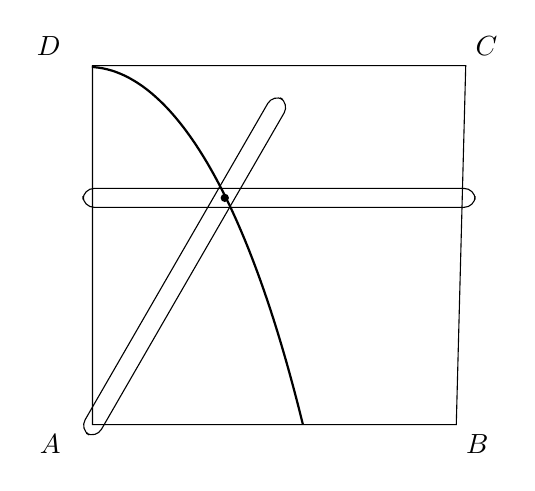
\begin{tikzpicture}[scale=.6,domain=.03:1.555,samples=100]
\draw (.1,.2) node[below left,xshift=-8pt] {$A$} -- (7.8,.2) node[below right] {$B$} -- (8,7.8) node[above right] {$C$} -- (.1,7.8) node[above left,xshift=-8pt] {$D$} -- cycle;
\draw[rounded corners,rotate=60] (0,-.2) rectangle (8.2,.2);
\draw[rounded corners] (-.1,4.8) rectangle (8.2,5.2);
\fill (2.9,5) circle [radius=2.5pt];
\draw[thick] plot (4.6*.637*\x,{12.2*.637*\x*cot(\x r)});
\end{tikzpicture}
\caption{Ein Quadratzirkel}\label{f.trisect-quad-compass}
\end{minipage}
\end{figure}

Eine Quadratrix kann mit Hilfe eines Quadratrix-Zirkels konstruiert werden, wie in Abb.~\ref{f.trisect-quad-compass} gezeigt. Er besteht aus zwei (unmarkierten) geraden Linien, die sich wie oben beschrieben bewegen. Ein Gelenk zwingt sie dazu, sich gemeinsam zu bewegen und zeichnet die Kurve nach.
\begin{figure}[b]
\begin{center}
\begin{tikzpicture}[scale=.8,domain=.03:1.562,samples=100]
\draw (.1,7.8) coordinate (start)
  node[above left] {$D$}
  node[below right,xshift=32pt] {$\theta$} -- 
  (.1,.2) node[below left] {$A$} -- 
  (8,.1)  node[below right] {$B$} -- 
  (8,7.8) node[above right] {$C$} -- 
  cycle;
\draw[name path=curve,thick] plot (4.6*.637*\x,{12.2*.637*\x*cot(\x r)});
% To ensure intersection at node D, path should extend to the upper left of D
\coordinate (twenty-a) at ($(start)+(-35:9)$);
\path[name path=twenty] ($(start)!-.1!(twenty-a)$) -- (twenty-a);
\path[name path=sixty] (start) -- +(-50:11);
\path[name path=xaxis] (.1,.2) -- (8,.1);
\path[name intersections={of=twenty and curve,by={x1,tri}}];
\draw (start) -- (tri);
\node[above right] at (tri) {$P_2$};
\path[name intersections={of=sixty and curve,by={x2,angle}}];
\node[above right] at (angle) {$P_1$};
\draw (start) -- (angle);
\path[name intersections={of=xaxis and curve,by=x}];
\path[name intersections={of=sixty and xaxis,by=sixty-x}];
\draw (start) -- (sixty-x);

\path (tri) -- (tri -| .1,.2) coordinate (t3);
\draw[dashed] (t3) -- +(7.9,0);
\node[left] at (t3) {$F$};
\path (angle) -- (angle -| .1,.2) coordinate (t);
\draw[dashed] (t) -- +(7.9,0);
\node[left] at (t) {$E$};
\draw[<->] (-1.2,7.8) -- node[fill=white] {$t/3$} (-1.2,7.8 |- t3);
\draw[<->] (-.6,7.8) -- node[fill=white] {$t$} (-.6,7.8 |- t);
\draw[<->] (-.6,7.8 |- t) -- node[fill=white] {$1-t$} (-.6,.2);
\draw (3.5,7.8) arc[start angle=0,delta angle=-49,radius=3.5];
\draw (1,7.8) arc[start angle=0,delta angle=-32,radius=1];
\node at (3.3,6) {$\alpha$}; 
\end{tikzpicture}
\end{center}
\caption{Dreiteilung eines Winkels mit Hilfe einer Quadratrix}\label{f.trisect-quad-trisect}
\end{figure}

Eine Quadratrix kann zur Dreiteilung eines Winkels verwendet werden.

\noindent\textbf{Konstruktion:}
Sei $\angle CDP_1=\alpha$ ein beliebiger Winkel, wobei $P_1$ der Schnittpunkt der Linie, die den Winkel $\alpha$ relativ zu $\overline{DC}$ definiert, mit der Quadratrix ist. Konstruieren Sie eine Linie durch $P_1$ parallel zu $\overline{DC}$ und bezeichnen Sie ihren Schnittpunkt mit $\overline{AD}$ als $E$. Bezeichne das Liniensegment $\overline{DE}$ mit $t$ und trisziere es (Sect.~\ref{s.trisect-constructible}), um den Punkt $F$ zu erhalten, der $t/3$ von $\overline{DC}$ entfernt ist. Sei $P_2$ der Schnittpunkt einer zu $\overline{DC}$ parallelen Linie von $F$ mit der Quadratrix, und bezeichne mit $\theta$ den Winkel zwischen $\overline{DC}$ und $\overline{DP_2}$ (Fig.~\ref{f.trisect-quad-trisect}).

\begin{theorem}
$\theta = \alpha/3$.
\end{theorem}
\begin{proof}
$E$ hat die $y$-Koordinate $1-t$, also hat $F$ konstruktionsbedingt die $y$-Koordinate $1-(t/3)$. Da die konstante lineare Geschwindigkeit der horizontalen Linie proportional zur konstanten Winkelgeschwindigkeit der rotierenden Linie $\theta/\alpha = (t/3)/t$ ist und $\theta = \alpha/3$.
\end{proof}

\section{Konstruierbare Zahlen}\label{s.trisect-constructible}
\index{Constructible number}

Sei $l$ ein Linienabschnitt der Länge $1$.

\begin{definition}
Eine Zahl $a$ ist dann und nur dann konstruierbar, wenn ein Linienabschnitt der Länge $a$ mit Lineal und Zirkel ausgehend von $l$ konstruiert werden kann.
\end{definition}

Konstruieren Sie für den Streckenabschnitt $l=\overline{AB}$ eine Linie, die $\overline{AB}$ enthält, und suchen Sie mit dem Zirkel einen Punkt $C$ auf der Linie, der $1$ von $B$ entfernt ist. Dann hat $\overline{AC}$ die Länge $2$, so dass die Zahl $2$ konstruierbar ist. Ein Linienabschnitt $\overline{BD}$ der Länge $1$ kann senkrecht zu $\overline{AB}$ bei $B$ konstruiert werden. Die Hypotenuse des Dreiecks $\triangle ABD$ hat die Länge $\sqrt{2}$, also ist die Zahl $\sqrt{2}$ konstruierbar.

\begin{theorem}\label{thm.trisect-constructible}
Eine Zahl ist dann und nur dann konstruierbar, wenn sie der Wert eines Ausdrucks ist, der aus den ganzen Zahlen, den vier arithmetischen Operationen $\{+,-,\times,/\}$ und der Operation der Quadratwurzel gebildet wird $\surd$.
\end{theorem}

\begin{proof}
Zunächst zeigen wir, dass die Werte dieser Ausdrücke konstruierbar sind.
\index{Constructible number!arithmetic operation}

\medskip

\begin{figure}[b]
\begin{center}
\begin{tikzpicture}[scale=.8]
\coordinate (P) at (0,0);
\coordinate (Q) at (5,0);
\coordinate (T) at (3,0);
\coordinate (U) at (7,0);
\vertex{P};
\vertex{Q};
\draw (P) -- (Q);
\node[above] at (P) {$P$};
\node[above left] at (Q) {$Q$};
\node[above left] at (U) {$U$};
\node[above right] at (T) {$T$};
\draw (5,0) -- (8,0);
\draw (5,0) circle[radius=2cm];
\draw (5,0) -- node[left] {$b$} ++(60:2cm);
\coordinate (R) at (9,-1);
\coordinate (S) at ($(9,-1) + (20:2cm)$);
\vertex{R};
\vertex{S};
\draw (R) node[above] {$R$} --
  node[below right] {$b$} (S)
  node[above] {$S$};
\draw[<->] (0,-.5) -- node[fill=white] {$a$} (5,-.5);
\draw[<->] (0,-1) -- node[fill=white] {$a-b$} (3,-1);
\draw[<->] (0,-1.5) -- node[fill=white] {$a+b$} (7,-1.5);
\end{tikzpicture}
\end{center}
\caption{Konstruktion von Addition und Subtraktion}\label{f.trisect-add-subtract}
\end{figure}

\noindent\textbf{Addition und Subtraktion:}
Konstruieren Sie aus den Linienabschnitten $\overline{PQ}=a$ und $\overline{RS}=b$ einen Kreis mit dem Mittelpunkt $Q$ und dem Radius $b$ (Abb.~\ref{f.trisect-add-subtract}). Verlängern Sie $\overline{PQ}$, bis sie den Kreis in $U$ schneidet. Dann ist $\overline{PTQU}$ ein Linienabschnitt, wobei $\overline{PT}=a-b$ und $\overline{PU}=a+b$.

\medskip

\noindent\textbf{Multiplication:}
By similar triangles in Fig.~\ref{f.trisect-multiplication},
$(1/b)=(a/\overline{OA})$, so $\overline{OA}=ab$.

\medskip

\noindent\textbf{Division:}
By similar triangles in Fig.~\ref{f.trisect-division},
$(1/b)=(\overline{OD}/a)$, so $\overline{OD}=(a/b)$.

\begin{figure}[t]
\begin{minipage}{.45\textwidth}
\begin{tikzpicture}[scale=.8]
\draw[name path=horz] (0,0) coordinate (o) -- (7,0);
\node[left] at (o) {$O$};
\coordinate (a) at (6,0);
\node[below]  at (a) {$A$};
\draw (o) -- (30:5.5);
\coordinate (c) at (30:3);
\coordinate (b) at (30:5);
\node[above] at (c) {$C$};
\node[above] at (b) {$B$};
\draw (a) -- (b);
\path[name path=par] (c) -- +($(a)-(b)$);
\path[name intersections={of=par and horz,by=d}];
\node[below] at (d) {$D$};
\draw (c) -- (d);
\draw[<->] (-.4,.5) -- node[fill=white] {$b$} +(30:5.2);
\path (o) -- node[above] {$1$} (c);
\draw[<->] (0,-.8) -- node[fill=white] {$ab$} +(6,0);
\path (o) -- node[below] {$a$} (d);
\end{tikzpicture}
\caption{Konstruktion der Multiplikation}\label{f.trisect-multiplication}
\end{minipage}
\hfill
\begin{minipage}{.45\textwidth}
\begin{tikzpicture}[scale=.8]
\draw[name path=horz] (0,0) coordinate (o) -- (7,0);
\node[left] at (o) {$O$};
\coordinate (a) at (6,0);
\node[below]  at (a) {$A$};
\draw (o) -- (30:5.5);
\coordinate (c) at (30:3);
\coordinate (b) at (30:5);
\node[above] at (c) {$C$};
\node[above] at (b) {$B$};
\draw (a) -- (b);
\path[name path=par] (c) -- +($(a)-(b)$);
\path[name intersections={of=par and horz,by=d}];
\node[below] at (d) {$D$};
\draw (c) -- (d);
\draw[<->] (-.4,.5) -- node[fill=white] {$b$} +(30:5.2);
\path (o) -- node[above] {$1$} (c);
\draw[<->] (0,-.8) -- node[fill=white] {$a$} +(6,0);
\path (o) -- node[below] {$a/b$} (d);
\end{tikzpicture}
\caption{Aufbau der Abteilung}\label{f.trisect-division}
\end{minipage}
\end{figure}

\medskip

\noindent\textbf{Quadratwurzeln:}
\index{Constructible number!square root}
Konstruieren Sie für ein Liniensegment $\overline{BC}=a$ $\overline{AB} =1+a$ und einen Halbkreis mit $\overline{AB}$ als Durchmesser. Konstruieren Sie eine Senkrechte bei $C$ und lassen Sie $D$ den Schnittpunkt der Senkrechten mit dem Kreis sein (Abb.~\ref{f.trisect-square-root}). $\angle ADB$ ist ein rechter Winkel, weil er durch einen Durchmesser begrenzt ist. Bei ähnlichen Dreiecken ist $(h/1)=(a/h)$, also $h^2=a$ und $h=\sqrt{a}$.

\begin{figure}[b]
\begin{center}
\begin{tikzpicture}[scale=1]
\draw[name path=horz] (0,0) coordinate (a) -- (6,0);
\node[left] at (a) {$A$};
\coordinate (b) at (6,0);
\node[below] at (b) {$B$};
\draw[name path=circle] (b) arc(0:180:3);
\path[name path=perp] (2,0) -- +(0,3.2);
\coordinate (c) at (2,0);
\node[below] at (c) {$C$};
\path[name intersections={of=circle and perp,by=d}];
\node[above] at (d) {$D$};
\draw (c) -- node[right] {$h$} (d);
\path (a) -- node[below] {$1$} (c) -- node[below] {$a$} (b);
\draw (c) rectangle +(6pt,6pt);
\draw (a) -- (d) -- (b);
\draw[rotate=-125] (d) rectangle +(6pt,6pt);
\node[above right,xshift=4pt] at (a) {$\alpha$};
\node[above left,xshift=-12pt] at (b) {$90^\circ\!-\!\alpha$};
\node[below right,yshift=-8pt] at (d) {$\alpha$};
\node[below left,xshift=0pt,yshift=-18pt] at (d) {$90^\circ\!-\!\alpha$};
\end{tikzpicture}
\end{center}
\caption{Konstruktion einer Quadratwurzel}
\label{f.trisect-square-root}
\end{figure}

\medskip

Um die Umkehrung des Satzes zu beweisen, müssen wir bestimmen, welche Ausdrücke mit Lineal und Zirkel konstruiert werden können. Es gibt drei Konstruktionen:\footnote{Aus Gründen der Übersichtlichkeit werden diese für bestimmte Werte und nicht für die allgemeinsten Gleichungen dargestellt.}

\begin{enumerate}
\item Zwei Linien schneiden sich in einem Punkt (Abb.~\ref{f.constructible-two-lines}). Die Koordinaten des Schnittpunktes lassen sich aus den Gleichungen der beiden Geraden ableiten
$y=x$ und $y=4x-2$. Der Schnittpunkt ist $P= (2/3, 2/3)$.

\item Eine Gerade schneidet einen Kreis in null, einem oder zwei Punkten (Abb.~\ref{f.constructible-line-circle}). Die Koordinaten der Schnittpunkte lassen sich aus den Gleichungen der Geraden $y=x$ und des Kreises $x^2+y^2=4$ ableiten. Die Schnittpunkte sind
$P=(\sqrt{2}, \sqrt{2})$ und $Q=(-\sqrt{2}, -\sqrt{2})$.

\item Zwei Kreise schneiden sich in null, einem oder zwei Punkten (Abb.~\ref{f.constructible-two-circles}). Die Koordinaten der Schnittpunkte lassen sich aus den Gleichungen der beiden Kreise $(x-1)^2+y^2=4$, $(x+1)^2+y^2=4$ ableiten. Die Schnittpunkte sind $P=(0,\sqrt{2}),Q=(0,-\sqrt{2})$.
\end{enumerate}
\end{proof}

\begin{figure}[t]
\begin{minipage}{.45\textwidth}
\begin{tikzpicture}[scale=.66]
\draw[step=10mm,white!50!black,very thin] (-4,-4) grid (4,4);
\draw[thick] (-4,0) -- (4,0);
\draw[thick] (0,-4) -- (0,4);
\coordinate (O) at (0,0);
\foreach \x in {-3,...,4}
  \node at (\x-.2,-.3) {\sm{\x}};
\foreach \y in {-3,...,-1}
  \node at (-.4,\y-.3) {\sm{\y}};
\foreach \y in {1,...,4}
  \node at (-.3,\y-.3) {\sm{\y}};
\draw[name path=eq1] (-4,-4) -- (4,4);
\draw[name path=eq2] (-.5,-4) -- (1.5,4);
\path[name intersections={of=eq1 and eq2,by={P}}];
\node[right] at (P) {$P$};
\end{tikzpicture}
\caption{Der Schnittpunkt von zwei Linien}\label{f.constructible-two-lines}
\end{minipage}
\hfill
\begin{minipage}{.45\textwidth}
\begin{tikzpicture}[scale=.66]
\coordinate (O) at (0,0);
\draw[step=10mm,white!50!black,very thin] (-4,-4) grid (4,4);
\draw[thick] (-4,0) -- (4,0);
\draw[thick] (0,-4) -- (0,4);
\foreach \x in {-3,...,4}
  \node at (\x-.2,-.3) {\sm{\x}};
\foreach \y in {-3,...,-1}
  \node at (-.4,\y-.3) {\sm{\y}};
\foreach \y in {1,...,4}
  \node at (-.3,\y-.3) {\sm{\y}};
\coordinate (A) at (2,0);
\node[draw,circle through=(A),name path=circle] at (0,0) {};
\draw[name path=eq1] (-4,-4) -- (4,4);
\path[name intersections={of=eq1 and circle,by={P,Q}}];
\node[right] at (P) {$P$};
\node[left] at (Q) {$Q$};
\end{tikzpicture}
\caption{Die Schnittpunkte einer Linie und eines Kreises}\label{f.constructible-line-circle}
\end{minipage}
\end{figure}


\begin{figure}[b]
\begin{center}
\begin{tikzpicture}[scale=.66]
\coordinate (O) at (0,0);
\draw[step=10mm,white!50!black,very thin] (-4,-4) grid (4,4);
\draw[thick] (-4,0) -- (4,0);
\draw[thick] (0,-4) -- (0,4);
\foreach \x in {-3,...,4}
  \node at (\x-.2,-.3) {\sm{\x}};
\foreach \y in {-3,...,-1}
  \node at (-.4,\y-.3) {\sm{\y}};
\foreach \y in {1,...,4}
  \node at (-.3,\y-.3) {\sm{\y}};
\coordinate (A) at (3,0);
\node[draw,circle through=(A),name path=circle1] at (1,0) {};
\coordinate (B) at (-3,0);
\node[draw,circle through=(B),name path=circle2] at (-1,0) {};
\path[name intersections={of=circle1 and circle2,by={P,Q}}];
\node[right,xshift=6pt,yshift=-2pt] at (P) {$P$};
\node[right,xshift=6pt,yshift=2pt] at (Q) {$Q$};
\end{tikzpicture}
\caption{Die Schnittpunkte von zwei Kreisen}\label{f.constructible-two-circles}
\end{center}
\end{figure}

\section{Konstruierbare Zahlen als Wurzeln von Polynomen}\label{s.trisect-poly}
Um zu zeigen, dass eine Zahl nicht konstruierbar ist, müssen wir beweisen, dass sie nicht nur mit ganzen Zahlen und den Operationen $\{+,-,\times,/,\surd\}$ ausgedrückt werden kann.

Wir werden zeigen, dass konstruierbare Zahlen die Wurzeln einer bestimmten Klasse von Polynomen sind, und dann beweisen, dass die Dreiteilung eines Winkels und die Verdopplung eines Würfels die Konstruktion von Wurzeln von Polynomen erfordern, die nicht zu dieser Klasse gehören. Heute werden diese Ergebnisse mit Hilfe der Feldtheorie der abstrakten Algebra bewiesen, aber hier gebe ich einen Beweis, der elementare Mathematik verwendet. Der Beweis basiert auf der folgenden Definition.

\begin{definition}
Die \emph{depth} eines Ausdrucks, der aus den ganzen Zahlen und den Operatoren $\{+,-,\times,/,\surd\}$ aufgebaut ist, ist die maximale Verschachtelungsebene von Quadratwurzeln.
\end{definition}\index{Konstruierbare Zahl!Tiefe von Quadratwurzeln}

\begin{example}
Betrachten Sie den folgenden Ausdruck:
\[
\sqrt{17+3\sqrt{17} - \sqrt{34-2\sqrt{17}}
  -2\sqrt{34+2\sqrt{17}} }\,.
\]
Die Tiefe beträgt $3$, weil rechts vom Ausdruck $\sqrt{17}$ steht, das in $\sqrt{34+2\sqrt{17}}$ verschachtelt ist, das wiederum in
$\sqrt{17+\cdots-\cdots-2\sqrt{34+2\sqrt{17}}}$
verschachtelt ist.
\end{example}

\begin{theorem}
Ein Ausdruck der Tiefe $n$ kann ausgedrückt werden als $a+b\sqrt{c}$, wobei $a,b,c$ Ausdrücke der Tiefe von höchstens $n-1$ sind.
\end{theorem}
\begin{proof}
Einfache Berechnungen zeigen, dass die Ausdrücke $(a_1+b_1\sqrt{c})\,\mathit{op}\,(a_2+b_2\sqrt{c})$ für die Operatoren $\mathit{op}=\{+,-,\times\}$ zu Ausdrücken $a+b\sqrt{c}$ der Tiefe $n-1$ führen. Bei der Division ist die Berechnung etwas komplizierter:
\begin{eqnarray*}
\frac{a_1+b_1\sqrt{c}}{a_2+b_2\sqrt{c}}&=&
\frac{(a_1+b_1\sqrt{c})(a_2-b_2\sqrt{c_2})}{(a_2+b_2\sqrt{c})(a_2-b_2\sqrt{c})}\\
&=&\frac{a_1a_2-b_1b_2c}{a_2^2-b_2^2c}+\frac{a_2b_1-a_1b_2}{a_2^2-b_2^2c}\sqrt{c}\,,
\end{eqnarray*}
die die Form $a+b\sqrt{c}$ hat, wobei $a,b,c$ die Tiefe $n-1$ haben. Schließlich ist die Quadratwurzel aus einem Ausdruck der Tiefe $n-1$ ein Ausdruck der Tiefe $n$.
\end{proof}


\begin{theorem}\label{thm.trisect.conjugate}
Sei $p(x)$ ein monisches kubisches Indexpolynom mit rationalen Koeffizienten:
\[
p(x)=x^3+a_2x^2+a_1x+a_0\,,
\]
und sei $r=a+b\sqrt{c}$ eine Wurzel von $p(x)$ \emph{von minimaler Tiefe} $n$, wobei $a,b,c$ (höchstens) $n-1$ tief sind. Dann ist $r'=a-b\sqrt{c}$ eine Wurzel von $p(x)$ und $r\neq r'$.
\end{theorem}\index{Roots!cubic@of cubic polynomials|(}

\begin{proof} Berechnen wir $p(r)$, das gleich $0$ ist, da $r$ eine Wurzel ist:
\[
\renewcommand{\arraystretch}{1.4}
\begin{array}{lcr}
(a+b\sqrt{c})^3+a_2(a+b\sqrt{c})^2+a_1(a+b\sqrt{c})+a_0&=\\
(a^3+3a^2b\sqrt{c}+3ab^2c+b^3c\sqrt{c})\\
\quad+\,a_2(a^2+2ab\sqrt{c}+b^2c) +a_1(a+b\sqrt{c}) +a_0&=\\
(a^3+3ab^2c+a_2a^2+a_2b^2c+a_1a+a_0)\\
\quad+\,(3a^2b+b^3c+2a_2ab+a_1b)\sqrt{c}&=\\
d+e\sqrt{c}&=&0\,.
\end{array}
\]
wobei $d,e$ Ausdrücke der Tiefe $n-1$ sind, die aus den rationalen Koeffizienten und $a,b,c$ gebildet werden. Dann ist $\sqrt{c}=-d/e$, so dass $a+b\sqrt{c}$ als Ausdruck der Tiefe $n-1$ ausgedrückt werden kann, wobei die Annahme gilt, dass $a+b\sqrt{c}$ von minimaler Tiefe $n$ ist. Da $\sqrt{c}\neq 0$ ist und die Tiefe $n$ hat, muss $d+e\sqrt{c}$ Null sein, damit $d=e=0$.

Betrachten wir nun $r'=a-b\sqrt{c}$. Aus der obigen Berechnung ergibt sich, dass $p(r')=d-e\sqrt{c}=0+0\cdot\sqrt{c}=0$, also ist auch $r'$ eine Wurzel aus $p$.

Wenn $r= r'$ ist, dann ist $0=r-r'=2b\sqrt{c}$, was nur gilt, wenn $b=0$ ist, so dass $r,r'$ die Tiefe $n-1$ hätte, was wiederum der Annahme widerspricht.
\end{proof}                                

\begin{theorem}
Wenn ein monisches Indexpolynom ein kubisches Polynom mit rationalen Koeffizienten ist:
\[p(x)=x^3+a_2x^2+a_1x+a_0\]
keine rationalen Wurzeln hat, ist keine seiner Wurzeln konstruierbar.
\end{theorem}

\begin{proof} Durch den Fundamentalsatz der Algebra\index{Fundamentalsatz der Algebra}  (Thm.~\ref{thm.fundamental}) hat $p(x)$ drei Wurzeln $r_1,r_2,r_3$. Sei $r_1=a+b\sqrt{c}$ eine Wurzel der minimalen Tiefe $n$. Unter der Annahme, dass es keine rationalen Wurzeln gibt, sei $n\geq 1$, und daher $b\neq 0$ und $c\neq 0$. Nach Thm.~\ref{thm.trisect.conjugate} ist $r_2=a-b\sqrt{c}$ ebenfalls eine Wurzel. Führen Sie die folgende Multiplikation durch:
\begin{subeqnarray}
(x-r_1)(x-r_2)(x-r_3)&=&x^3 -(r_1+r_2+r_3)x^2\\
&&\quad\; +\, (r_1r_2+r_1r_3+r_2r_3)x + r_1r_2r_3\slabel{eq.viete3}\\
a_2&=&-(r_1+r_2+r_3)\\
r_3&=&-(a_2+r_1+r_2)\,.
\end{subeqnarray}
Da $a_2$ rational ist, ist es das auch:
\[r_3=-a_2-(r_1+r_2)=-a_2-2a\,,\]
was der Annahme widerspricht.
\end{proof}
\index{Roots!cubic@of cubic polynomials|)}

\section{Die Unmöglichkeit der klassischen Konstruktionen}\label{s.trisect-impossible}

\begin{theorem}\label{thm.trisect.cube-root-irrational}
$\sqrt[3]{2}$ ist irrational.
\end{theorem}
\begin{proof}
Nehmen wir an, dass $\sqrt[3]{2}$ rational und gleich $p/q$ ist, wobei $p,q$ ganze Zahlen sind, die keine anderen gemeinsamen Faktoren als $\pm 1$ haben. Dann:
\begin{eqnarray*}
(p/q)^3&=&(\sqrt[3]{2})^3\\
p^3&=&2q^3\,,
\end{eqnarray*}
also muss $p$ durch $2$ teilbar sein, also $p=2r$. Jetzt:
\begin{eqnarray*}
8r^3&=&2q^3\\
q^3&=&4r^3\,,
\end{eqnarray*}
$q$ ist also durch $2$ teilbar, was der Annahme widerspricht, dass $p,q$ keinen gemeinsamen Faktor haben.
\end{proof}

\begin{theorem}
$x^3-2$ hat keine rationalen Wurzeln, so dass es unmöglich ist, einen Würfel mit Lineal und Zirkel zu verdoppeln.\index{Doubling a cube!impossibility of}
\end{theorem}
\begin{proof} Eine seiner Wurzeln ist $\sqrt[3]{2}$, die nach Thm.~\ref{thm.trisect.cube-root-irrational} irrational ist. Die anderen Wurzeln sind die Wurzeln der quadratischen Gleichung $x^2+\sqrt[3]{2}x+(\sqrt[3]{2})^2$, die man durch Division von $x^3-2$ durch $x-\sqrt[3]{2}$ erhält. Es ist leicht zu überprüfen, dass die Wurzeln nicht rational sind (tatsächlich nicht einmal real).
\end{proof}

\begin{theorem}
Es ist unmöglich, einen beliebigen Winkel mit einem Lineal und einem Zirkel zu dreiteilen.
\end{theorem}
\begin{proof}
Es genügt, die Unmöglichkeit für einen Winkel zu zeigen. Versuchen wir, $60^\circ$ zu dreiteilen, um $20^\circ$ zu erhalten.
\index{Trisection of an angle!impossibility of}
Nach Thm.~\ref{thm.triple-angle}:
\begin{eqnarray*}
\cos 3\alpha&=&4\cos^3\alpha -3\cos\alpha\\
\cos 60^\circ&=&4\cos^3 20^\circ -3\cos 20^\circ\,.
\end{eqnarray*}
Bezeichne $x=\cos 20^\circ$ und $2x$ durch $y$. Da $\cos 60^\circ=1/2$ ist, haben wir:
\begin{eqnarray*}
4x^3 -3x-\frac{1}{2} &=& 0\\
8x^3-6x-1&=&0\\
y^3-3y-1&=&0\,.
\end{eqnarray*}

Um zu beweisen, dass das Polynom $y^3-3y-1$ keine rationalen Wurzeln hat, nehme man an, dass $y=a/b$ eine rationale Wurzel ist, wobei $a,b$ keinen anderen gemeinsamen Faktor als $\pm 1$ haben. Dann:
\begin{subeqnarray}
(a/b)^3-3(a/b)-1&=&0\\
a^3-3ab^2&=&b^3\\
a(a-3b^2)&=&b^3\slabel{eq.trisect1}\\
a^3&=&b(b^2+3ab)\slabel{eq.trisect2}\,.
\end{subeqnarray}
Nach Gl.~\ref{eq.trisect1} muss $b$ durch $a$ teilbar sein, und nach Gl.~\ref{eq.trisect2} muss $a$ durch $b$ teilbar sein, was nur möglich ist, wenn $a=b=\pm 1$ und $a/b=\pm 1$. Rein rechnerisch sind $y=a/b=1$ und $y=a/b=-1$ keine Wurzeln des Polynoms.
\end{proof}
Ein alternativer Weg, die Unmöglichkeit der Konstruktionen zu beweisen, ist die Verwendung des folgenden Satzes, den wir ohne Beweis präsentieren.

\begin{theorem}\label{thm.factor}
Wenn ein monisches Indexpolynom $p(x)=x^n+a_{n-1}x^{n-1}+\cdots+a_0$ mit ganzzahligen Koeffizienten rationale Wurzeln hat, dann hat es ganzzahlige Wurzeln.
\end{theorem}

Um zu zeigen, dass es nicht möglich ist, einen Würfel zu duplizieren, müssen wir zeigen, dass:
\[
x^3-2=(x-r_2)(x-r_1)(x-r_0)
\]
hat keine ganzzahligen Wurzeln. Da $r_0r_1r_2=-2$ ist, müssen alle Wurzeln durch $2$ geteilt werden, also sind die einzigen möglichen ganzzahligen Wurzeln $\pm 1, \pm 2$. Eine schnelle Berechnung zeigt, dass keine von ihnen Wurzeln sind.

Um die Unmöglichkeit der Dreiteilung eines Winkels zu zeigen, müssen wir zeigen, dass $y^3-3y-1$ keine ganzzahligen Wurzeln hat. Eine ganzzahlige Wurzel muss $-1$ teilen, aber weder $1$ noch $-1$ sind Wurzeln.

\subsection*{What Is the Surprise?}

Underwood Dudley hat eine umfangreiche Studie über die, wie er sie nennt, ``Cranks'' durchgeführt, die Jahre ihres Lebens mit dem Versuch verschwenden, Winkel mit Lineal und Zirkel zu verdrehen. Sie machen sich nicht nur vor, daß dies möglich ist, sondern, was noch schlimmer ist, sie glauben, daß eine Lösung wichtig wäre. Natürlich hätte eine Lösung keinen praktischen Nutzen, da Werkzeuge wie die Neusis und die Quadratrix das Problem exakt lösen können. Die schiere Anzahl solcher Konstruktionen ist erstaunlich, zumal viele von ihnen clever sind und gute Näherungen erzielen. Das Berechnen der mit den Konstruktionen verbundenen Formeln ist eine hervorragende Übung in Trigonometrie.

Erstaunlich ist auch, dass die Beweise für die Unmöglichkeit dieser geometrischen Konstruktionen rein algebraisch sind, indem man die Eigenschaften der Wurzeln von Polynomen verwendet.

\subsection*{Quellen}

Wikipedia \cite{wiki:tri, wiki:neu, wiki:quad} ist eine gute Quelle für die Konstruktionen in diesem Kapitel.
Die beiden angenäherten Dreiteilungen stammen aus \cite[pp.
~67--68, 95--96]{dudley-budget}. Das zweite Beispiel wird dem berühmten Philosophen Thomas Hobbes zugeschrieben. Sowohl \cite[pp.~48--49]{martin} als auch \cite[pp.~6--7]{dudley-budget} behandeln die Dreiteilung mit Hilfe der Quadratrix.
Die Verdoppelung des Würfels mit Hilfe einer Neusis wird von \cite{dorrie2} übernommen.

Eine rigorose Behandlung der Konstruierbarkeit findet sich in Lehrbüchern über abstrakte Algebra wie \cite{fraleigh}, das einen allgemeinen Beweis der Umkehrung von Thm~\ref{thm.trisect-constructible} in Sect.~32 enthält.
Theorem~\ref{thm.factor} ist Thm.~23.11 von \cite{fraleigh}.
Eine relativ zugängliche Darstellung von Wantzels Beweis findet sich in \cite{suzuki}. Meine Darstellung der Konstruierbarkeit stützt sich auf die Darstellungen in \cite[Kap.~III]{courant} und \cite{laugwitz}.

